\documentclass[a4paper,12pt]{article}
\usepackage[croatian]{babel}
\usepackage[utf8]{inputenc}
\usepackage{amsmath,amssymb}
\usepackage{graphicx}
\usepackage{xcolor}
\usepackage{tabularx}
\usepackage{lipsum}
\usepackage[useregional]{datetime2}
\usepackage{url}

\addtolength{\voffset}{-2cm} \addtolength{\textheight}{4cm}
\addtolength{\hoffset}{-1cm} \addtolength{\textwidth}{2cm}
\selectlanguage{croatian}

\newcommand*{\devname}{\texttt}
\newcommand*{\techspec}{\textsc}
\newcommand*{\term}{\textit}
\newcommand{\sitename}[1]{\texttt{"#1"}}
\renewcommand*{\emph}{\textbf}

\newcommand*{\maketitlepage}{%intro
  \begin{center}
    Sveučilište u Splitu\\
    Prirodoslovno-matematički fakultet\\
    Odjel za fiziku

    \bigskip
    \bigskip

    \large{Programski alati u fizici}


    \bigskip
    \bigskip

    \textbf{{\Large{Brojanje zvijezda na noćnom nebu}}}
  \end{center}
  \begin{center}
    \textbf{Frane Doljanin}\\
    \
  \end{center}
  \begin{center}
    Split, \DTMdate{2023-6-8}
  \end{center}
}


\begin{document}

\frame{\titlepage}

\begin{frame}
  \frametitle{Motivacija}
  \begin{minipage}{0.55\linewidth}
    Zvijezde na noćnom nebu...\newline \pause
    Baza podataka VizieR,\\ satelit Hipparcos:\pause
    \begin{itemize}
      \item 118 218 zvijezda
      \item 1989. - 1993.
      \item 51MB
    \end{itemize}
    \pause
  \end{minipage}
  \begin{minipage}{0.40\linewidth}
    \begin{figure}
      \centering
      
\includegraphics[width=\textwidth]{assets/prez-starry_night.png}
      \caption{DALL-E o PMF noćima} \label{fig:starry_night}
    \end{figure}
  \end{minipage}
\end{frame}

\begin{frame}
  \frametitle{Teorija iza problema}
  Da bismo mogli brojati zvijezde, moramo znati jesu li oku vidljive i ispod/iznad horizonta.\\ \pause
  Koristimo sljedeća svojstva:
  \begin{itemize}
    \item rektascenzija i deklinacija
    \item azimut i elevacija
    \item prividna magnituda
  \end{itemize}
  \pause
  \medskip
  \begin{alertblock}{Ograničenja}
    Ovakav pristup ne uzima u obzir atmosferske uvjete, svjetlosno zagađenje, reljef...
  \end{alertblock}
\end{frame}

\begin{frame}
  \frametitle{Teorija iza problema}
  \begin{figure}[h]
    \begin{minipage}[t]{0.43\linewidth}
      \centering
      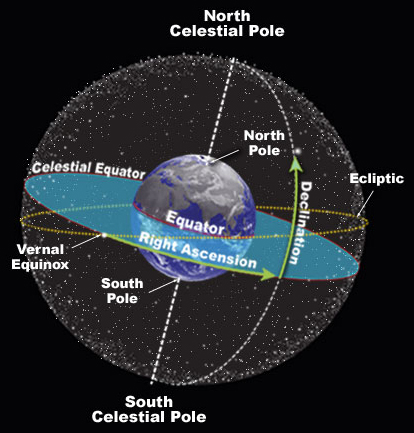
\includegraphics[height=128px]{assets/ext-ra_de.jpg}
      \caption{Prikaz nebeskih koordinata - rektascenzija i deklinacija.}\label{fig:ra_de}
    \end{minipage}
    \begin{minipage}[t]{0.55\linewidth}
      \centering
      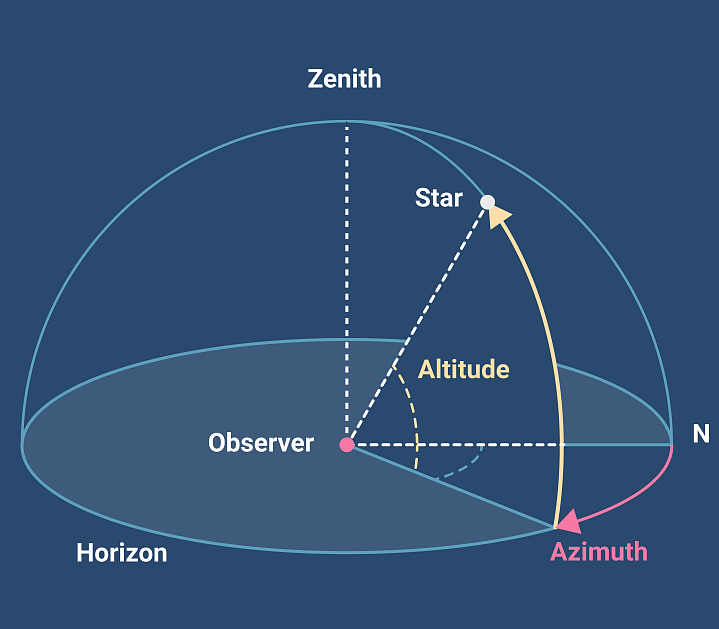
\includegraphics[height=128px]{assets/ext_el-as.png}
      \caption{Elevacija (altitude) i azimut.}\label{fig:el_as}
    \end{minipage}
  \end{figure}
\end{frame}

\begin{frame}
  \frametitle{Kôd}
  \pause ... je kod mene
\end{frame}

\begin{frame}
  \frametitle{Hvala na pažnji!}
\end{frame}

\end{document}